\begin{frame}[squeeze]{Złożoność obliczeniowa}

    \begin{figure}[H]
        \centering
        \begin{minipage}[t]{0.45\textwidth}
            \centering
            \fbox{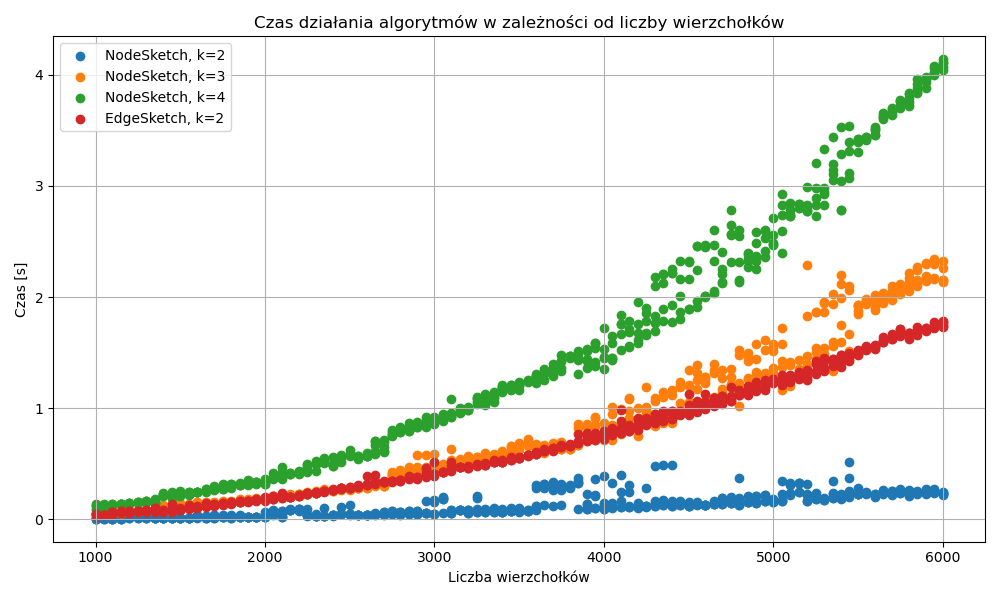
\includegraphics[width=\textwidth]{./img/time_all.png}}
            \caption{Czas działania algorytmów w zależności od liczby wierzchołków.}
        \end{minipage}
        \hspace{0.03\textwidth}
        \begin{minipage}[t]{0.45\textwidth}
            \centering
            \fbox{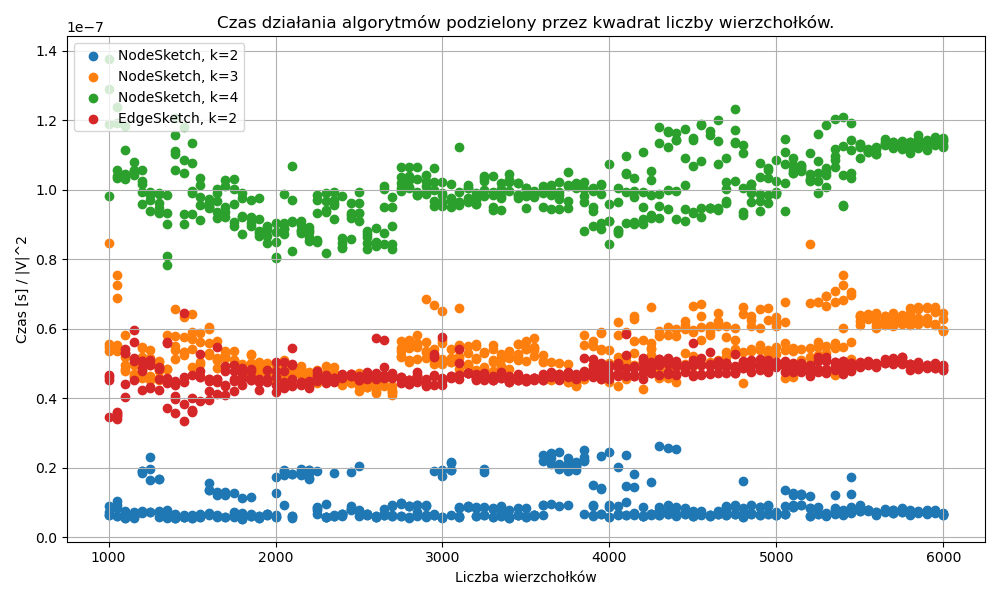
\includegraphics[width=\textwidth]{./img/time_normalized.png}}
            \caption{Czas działania algorytmów podzielony przez kwadrat liczby wierzchołków.}
        \end{minipage}
    \end{figure} 
\end{frame}